%%
%% Automatically generated file from DocOnce source
%% (https://github.com/hplgit/doconce/)
%%

% #define PREAMBLE

% #ifdef PREAMBLE
%-------------------- begin preamble ----------------------

\documentclass[%
oneside,                 % oneside: electronic viewing, twoside: printing
final,                   % draft: marks overfull hboxes, figures with paths
10pt]{article}

\listfiles               % print all files needed to compile this document

\usepackage{relsize,makeidx,color,setspace,amsmath,amsfonts,amssymb}
\usepackage[table]{xcolor}
\usepackage{bm,microtype}

\usepackage[pdftex]{graphicx}

% Packages for typesetting blocks of computer code
\usepackage{fancyvrb,framed,moreverb}

% Define colors
\definecolor{orange}{cmyk}{0,0.4,0.8,0.2}
\definecolor{tucorange}{rgb}{1.0,0.64,0}
\definecolor{darkorange}{rgb}{.71,0.21,0.01}
\definecolor{darkgreen}{rgb}{.12,.54,.11}
\definecolor{myteal}{rgb}{.26, .44, .56}
\definecolor{gray}{gray}{0.45}
\definecolor{mediumgray}{gray}{.8}
\definecolor{lightgray}{gray}{.95}
\definecolor{brown}{rgb}{0.54,0.27,0.07}
\definecolor{purple}{rgb}{0.5,0.0,0.5}
\definecolor{darkgray}{gray}{0.25}
\definecolor{darkblue}{rgb}{0,0.08,0.45}
\definecolor{darkblue2}{rgb}{0,0,0.8}
\definecolor{lightred}{rgb}{1.0,0.39,0.28}
\definecolor{lightgreen}{rgb}{0.48,0.99,0.0}
\definecolor{lightblue}{rgb}{0.53,0.81,0.92}
\definecolor{lightblue2}{rgb}{0.3,0.3,1.0}
\definecolor{lightpurple}{rgb}{0.87,0.63,0.87}
\definecolor{lightcyan}{rgb}{0.5,1.0,0.83}

\colorlet{comment_green}{green!50!black}
\colorlet{string_red}{red!60!black}
\colorlet{keyword_pink}{magenta!70!black}
\colorlet{indendifier_green}{green!70!white}

% Backgrounds for code
\definecolor{cbg_gray}{rgb}{.95, .95, .95}
\definecolor{bar_gray}{rgb}{.92, .92, .92}

\definecolor{cbg_yellowgray}{rgb}{.95, .95, .85}
\definecolor{bar_yellowgray}{rgb}{.95, .95, .65}

\colorlet{cbg_yellow2}{yellow!10}
\colorlet{bar_yellow2}{yellow!20}

\definecolor{cbg_yellow1}{rgb}{.98, .98, 0.8}
\definecolor{bar_yellow1}{rgb}{.98, .98, 0.4}

\definecolor{cbg_red1}{rgb}{1, 0.85, 0.85}
\definecolor{bar_red1}{rgb}{1, 0.75, 0.85}

\definecolor{cbg_blue1}{rgb}{0.87843, 0.95686, 1.0}
\definecolor{bar_blue1}{rgb}{0.7,     0.95686, 1}

%\setlength{\fboxsep}{-1.5mm}  % adjust cod_vpad/pro_vpad background box

%% Background for code blocks (parameter is color name)

%% pro/cod_vpad: gives some vertical padding before and after the text
%% (but has more simplistic code than _cod/pro_tight+cod/pro).
%% pro/cod_vpad can be used to enclose Verbatim or lst begin/end for code.
%% pro/cod calls _pro/cod_tight and has very little vertical padding,
%% used to enclose Verbatim and other begin/end for code.
%% (pro/cod is what the ptex2tex program could produce with the
%% Blue/BlueBar definitions in .ptex2tex.cfg.)

\newenvironment{cod_vpad}[1]{
   \def\FrameCommand{\colorbox{#1}}
   \MakeFramed{\FrameRestore}}
   {\endMakeFramed}

\newenvironment{_cod_tight}[1]{
   \def\FrameCommand{\colorbox{#1}}
   \FrameRule0.6pt\MakeFramed {\FrameRestore}\vskip3mm}
   {\vskip0mm\endMakeFramed}

\newenvironment{cod}[1]{
\bgroup\rmfamily
\fboxsep=0mm\relax
\begin{_cod_tight}{#1}
\list{}{\parsep=-2mm\parskip=0mm\topsep=0pt\leftmargin=2mm
\rightmargin=2\leftmargin\leftmargin=4pt\relax}
\item\relax}
{\endlist\end{_cod_tight}\egroup}

%% Background for complete program blocks (parameter 1 is color name
%% for background, parameter 2 is color for left bar)
\newenvironment{pro_vpad}[2]{
   \def\FrameCommand{\color{#2}\vrule width 1mm\normalcolor\colorbox{#1}}
   \MakeFramed{\FrameRestore}}
   {\endMakeFramed}

\newenvironment{_pro_tight}[2]{
   \def\FrameCommand{\color{#2}\vrule width 1mm\normalcolor\colorbox{#1}}
   \FrameRule0.6pt\MakeFramed {\advance\hsize-2mm\FrameRestore}\vskip3mm}
   {\vskip0mm\endMakeFramed}

\newenvironment{pro}[2]{
\bgroup\rmfamily
\fboxsep=0mm\relax
\begin{_pro_tight}{#1}{#2}
\list{}{\parsep=-2mm\parskip=0mm\topsep=0pt\leftmargin=2mm
\rightmargin=2\leftmargin\leftmargin=4pt\relax}
\item\relax}
{\endlist\end{_pro_tight}\egroup}


\usepackage[T1]{fontenc}
%\usepackage[latin1]{inputenc}
\usepackage{ucs}
\usepackage[utf8x]{inputenc}

\usepackage{lmodern}         % Latin Modern fonts derived from Computer Modern

% Hyperlinks in PDF:
\definecolor{linkcolor}{rgb}{0,0,0.4}
\usepackage{hyperref}
\hypersetup{
    breaklinks=true,
    colorlinks=true,
    linkcolor=linkcolor,
    urlcolor=linkcolor,
    citecolor=black,
    filecolor=black,
    %filecolor=blue,
    pdfmenubar=true,
    pdftoolbar=true,
    bookmarksdepth=3   % Uncomment (and tweak) for PDF bookmarks with more levels than the TOC
    }
%\hyperbaseurl{}   % hyperlinks are relative to this root

\setcounter{tocdepth}{2}  % number chapter, section, subsection

% Tricks for having figures close to where they are defined:
% 1. define less restrictive rules for where to put figures
\setcounter{topnumber}{2}
\setcounter{bottomnumber}{2}
\setcounter{totalnumber}{4}
\renewcommand{\topfraction}{0.95}
\renewcommand{\bottomfraction}{0.95}
\renewcommand{\textfraction}{0}
\renewcommand{\floatpagefraction}{0.75}
% floatpagefraction must always be less than topfraction!
% 2. ensure all figures are flushed before next section
\usepackage[section]{placeins}
% 3. enable begin{figure}[H] (often leads to ugly pagebreaks)
%\usepackage{float}\restylefloat{figure}

\usepackage[framemethod=TikZ]{mdframed}

% --- begin definitions of admonition environments ---

% Admonition style "mdfbox" is an oval colored box based on mdframed
% "notice" admon
\colorlet{mdfbox_notice_background}{gray!5}
\newmdenv[
  skipabove=15pt,
  skipbelow=15pt,
  outerlinewidth=0,
  backgroundcolor=mdfbox_notice_background,
  linecolor=black,
  linewidth=2pt,       % frame thickness
  frametitlebackgroundcolor=blue!5,
  frametitlerule=true,
  frametitlefont=\normalfont\bfseries,
  shadow=false,        % frame shadow?
  shadowsize=11pt,
  leftmargin=0,
  rightmargin=0,
  roundcorner=5,
  needspace=0pt,
]{notice_mdfboxmdframed}

\newenvironment{notice_mdfboxadmon}[1][]{
\begin{notice_mdfboxmdframed}[frametitle=#1]
}
{
\end{notice_mdfboxmdframed}
}

% Admonition style "mdfbox" is an oval colored box based on mdframed
% "summary" admon
\colorlet{mdfbox_summary_background}{gray!5}
\newmdenv[
  skipabove=15pt,
  skipbelow=15pt,
  outerlinewidth=0,
  backgroundcolor=mdfbox_summary_background,
  linecolor=black,
  linewidth=2pt,       % frame thickness
  frametitlebackgroundcolor=blue!5,
  frametitlerule=true,
  frametitlefont=\normalfont\bfseries,
  shadow=false,        % frame shadow?
  shadowsize=11pt,
  leftmargin=0,
  rightmargin=0,
  roundcorner=5,
  needspace=0pt,
]{summary_mdfboxmdframed}

\newenvironment{summary_mdfboxadmon}[1][]{
\begin{summary_mdfboxmdframed}[frametitle=#1]
}
{
\end{summary_mdfboxmdframed}
}

% Admonition style "mdfbox" is an oval colored box based on mdframed
% "warning" admon
\colorlet{mdfbox_warning_background}{gray!5}
\newmdenv[
  skipabove=15pt,
  skipbelow=15pt,
  outerlinewidth=0,
  backgroundcolor=mdfbox_warning_background,
  linecolor=black,
  linewidth=2pt,       % frame thickness
  frametitlebackgroundcolor=blue!5,
  frametitlerule=true,
  frametitlefont=\normalfont\bfseries,
  shadow=false,        % frame shadow?
  shadowsize=11pt,
  leftmargin=0,
  rightmargin=0,
  roundcorner=5,
  needspace=0pt,
]{warning_mdfboxmdframed}

\newenvironment{warning_mdfboxadmon}[1][]{
\begin{warning_mdfboxmdframed}[frametitle=#1]
}
{
\end{warning_mdfboxmdframed}
}

% Admonition style "mdfbox" is an oval colored box based on mdframed
% "question" admon
\colorlet{mdfbox_question_background}{gray!5}
\newmdenv[
  skipabove=15pt,
  skipbelow=15pt,
  outerlinewidth=0,
  backgroundcolor=mdfbox_question_background,
  linecolor=black,
  linewidth=2pt,       % frame thickness
  frametitlebackgroundcolor=blue!5,
  frametitlerule=true,
  frametitlefont=\normalfont\bfseries,
  shadow=false,        % frame shadow?
  shadowsize=11pt,
  leftmargin=0,
  rightmargin=0,
  roundcorner=5,
  needspace=0pt,
]{question_mdfboxmdframed}

\newenvironment{question_mdfboxadmon}[1][]{
\begin{question_mdfboxmdframed}[frametitle=#1]
}
{
\end{question_mdfboxmdframed}
}

% Admonition style "mdfbox" is an oval colored box based on mdframed
% "block" admon
\colorlet{mdfbox_block_background}{gray!5}
\newmdenv[
  skipabove=15pt,
  skipbelow=15pt,
  outerlinewidth=0,
  backgroundcolor=mdfbox_block_background,
  linecolor=black,
  linewidth=2pt,       % frame thickness
  frametitlebackgroundcolor=blue!5,
  frametitlerule=true,
  frametitlefont=\normalfont\bfseries,
  shadow=false,        % frame shadow?
  shadowsize=11pt,
  leftmargin=0,
  rightmargin=0,
  roundcorner=5,
  needspace=0pt,
]{block_mdfboxmdframed}

\newenvironment{block_mdfboxadmon}[1][]{
\begin{block_mdfboxmdframed}[frametitle=#1]
}
{
\end{block_mdfboxmdframed}
}

% --- end of definitions of admonition environments ---

% prevent orhpans and widows
\clubpenalty = 10000
\widowpenalty = 10000

\newenvironment{doconceexercise}{}{}
\newcounter{doconceexercisecounter}
% --- begin definition of \listofexercises command ---
\makeatletter
\newcommand\listofexercises{\section*{List of Exercises, Problems, and Projects}
\@starttoc{loe}
}
\newcommand*{\l@doconceexercise}{\@dottedtocline{0}{0pt}{6.5em}}
\makeatother
% --- end definition of \listofexercises command ---



% ------ header in subexercises ------
%\newcommand{\subex}[1]{\paragraph{#1}}
%\newcommand{\subex}[1]{\par\vspace{1.7mm}\noindent{\bf #1}\ \ }
\makeatletter
% 1.5ex is the spacing above the header, 0.5em the spacing after subex title
\newcommand\subex{\@startsection{paragraph}{4}{\z@}%
                  {1.5ex\@plus1ex \@minus.2ex}%
                  {-0.5em}%
                  {\normalfont\normalsize\bfseries}}
\makeatother


% --- end of standard preamble for documents ---


% insert custom LaTeX commands...

\raggedbottom
\makeindex
\usepackage[totoc]{idxlayout}   % for index in the toc
\usepackage[nottoc]{tocbibind}  % for references/bibliography in the toc

%-------------------- end preamble ----------------------

\begin{document}

% matching end for #ifdef PREAMBLE
% #endif

\newcommand{\half}{\frac{1}{2}}
\newcommand{\halfi}{{1/2}}
\newcommand{\tp}{\thinspace .}

\newcommand{\uex}{{u_{\small\mbox{e}}}}
\newcommand{\uexd}[1]{{u_{\small\mbox{e}, #1}}}
\newcommand{\vex}{{v_{\small\mbox{e}}}}
\newcommand{\vexd}[1]{{v_{\small\mbox{e}, #1}}}
\newcommand{\Aex}{{A_{\small\mbox{e}}}}

% Operators
\newcommand{\Ddt}[1]{\frac{D #1}{dt}}
\newcommand{\E}[1]{\hbox{E}\lbrack #1 \rbrack}
\newcommand{\Var}[1]{\hbox{Var}\lbrack #1 \rbrack}
\newcommand{\Std}[1]{\hbox{Std}\lbrack #1 \rbrack}

\newcommand{\xpoint}{\bm{x}}
\newcommand{\normalvec}{\bm{n}}
\newcommand{\Oof}[1]{\mathcal{O}(#1)}

% Boldface vectors/tensors
\newcommand{\x}{\bm{x}}
\newcommand{\X}{\bm{X}}
\renewcommand{\u}{\bm{u}}
\renewcommand{\v}{\bm{v}}
\newcommand{\w}{\bm{w}}
\newcommand{\acc}{\bm{a}}
\newcommand{\rpos}{\bm{r}}
\newcommand{\V}{\bm{V}}
\newcommand{\e}{\bm{e}}
\newcommand{\f}{\bm{f}}
\newcommand{\F}{\bm{F}}
\newcommand{\stress}{\bm{\sigma}}
\newcommand{\strain}{\bm{\varepsilon}}
\newcommand{\stressc}{{\sigma}}
\newcommand{\strainc}{{\varepsilon}}
\newcommand{\I}{\bm{I}}
\newcommand{\T}{\bm{T}}

\newcommand{\dfc}{\alpha}  % diffusion coefficient
% Unit vectors
\newcommand{\ii}{\bm{i}}
\newcommand{\jj}{\bm{j}}
\newcommand{\kk}{\bm{k}}
\newcommand{\ir}{\bm{i}_r}
\newcommand{\ith}{\bm{i}_{\theta}}
\newcommand{\iz}{\bm{i}_z}

% Index sets
\newcommand{\Ix}{\mathcal{I}_x}
\newcommand{\Iy}{\mathcal{I}_y}
\newcommand{\Iz}{\mathcal{I}_z}
\newcommand{\It}{\mathcal{I}_t}
%\newcommand{\Ix}{{I_x}}
%\newcommand{\Iy}{{I_y}}
%\newcommand{\Iz}{{I_z}}
%\newcommand{\It}{{I_t}}
%\newcommand{\If}{\mathcal{I}}     % for FEM
\newcommand{\If}{\mathcal{I}_s}     % for FEM
%\newcommand{\If}{{I}}     % for FEM
%\newcommand{\Ifd}{\mathcal{I}_d}  % for FEM
\newcommand{\Ifd}{{I_d}}  % for FEM
\newcommand{\Ifb}{{I_b}}  % for FEM
\newcommand{\setb}[1]{#1^0}    % set begin
\newcommand{\sete}[1]{#1^{-1}} % set end
%\newcommand{\setl}[1]{#1\setminus\{\set1{#1}\}}
%\newcommand{\setr}[1]{#1\setminus\{\set0{#1}\}}
%\newcommand{\seti}[1]{#1\setminus\{\set0{#1},\set1{#1}\}}
\newcommand{\setl}[1]{#1^-}
\newcommand{\setr}[1]{#1^+}
\newcommand{\seti}[1]{#1^i}
\newcommand{\sequencei}[1]{\left\{ {#1}_i \right\}_{i\in\If}}

% Finite elements
\newcommand{\basphi}{\varphi}
\newcommand{\baspsi}{\psi}
\newcommand{\refphi}{\tilde\basphi}
\newcommand{\psib}{\bm{\psi}}
\newcommand{\sinL}[1]{\sin\left((#1+1)\pi\frac{x}{L}\right)}
\newcommand{\xno}[1]{x_{#1}}
%\newcommand{\xno}[1]{x^{(#1)}}
\newcommand{\Xno}[1]{X_{(#1)}}
\newcommand{\yno}[1]{y_{#1}}
\newcommand{\Yno}[1]{Y_{(#1)}}
\newcommand{\xdno}[1]{\bm{x}_{#1}}

% FEniCS commands
\newcommand{\dX}{\, \mathrm{d}X}
\newcommand{\dx}{\, \mathrm{d}x}
\newcommand{\ds}{\, \mathrm{d}s}
\newcommand{\Real}{\mathbb{R}}
\newcommand{\Integerp}{\mathbb{N}}
\newcommand{\Integer}{\mathbb{Z}}


% ------------------- main content ----------------------



% ----------------- title -------------------------

\thispagestyle{empty}

\begin{center}
{\LARGE\bf
\begin{spacing}{1.25}
Generalizations of exponential decay models
\end{spacing}
}
\end{center}

% ----------------- author(s) -------------------------

\begin{center}
{\bf Hans Petter Langtangen${}^{1, 2}$} \\ [0mm]
\end{center}

\begin{center}
% List of all institutions:
\centerline{{\small ${}^1$Center for Biomedical Computing, Simula Research Laboratory}}
\centerline{{\small ${}^2$Department of Informatics, University of Oslo}}
\end{center}
    
% ----------------- end author(s) -------------------------

% --- begin date ---
\begin{center}
Oct 10, 2015
\end{center}
% --- end date ---

\vspace{1cm}


\tableofcontents

\clearpage % pagebreak before list of exercises
\subsection*{List of Exercises, Problems, and Projects}
\begin{tabular}{lrll}
Exercise & 1 & Experiment with precision in tests and the ... & p.~\pageref{decay:fd2:exer:precision} \\
Exercise & 2 & Implement the 2-step backward scheme & p.~\pageref{decay:fd2:exer:bw2} \\
Exercise & 3 & Implement the 2nd-order Adams-Bashforth scheme ... & p.~\pageref{decay:fd2:exer:AB2} \\
Exercise & 4 & Implement the 3rd-order Adams-Bashforth scheme ... & p.~\pageref{decay:fd2:exer:AB3} \\
Exercise & 5 & Analyze explicit 2nd-order methods & p.~\pageref{decay:exer:RK2:Taylor:analysis} \\
Project & 6 & Implement and investigate the Leapfrog scheme & p.~\pageref{decay:fd2:exer:leapfrog1} \\
Problem & 7 & Make a unified implementation of many schemes & p.~\pageref{decay:fd2:exer:uni} \\
\end{tabular}
% --- end of table of exercises
\clearpage % pagebreak after list of exercises




\vspace{1cm} % after toc







% !split
\section{Model extensions}

This section looks at the generalizations to $u^{\prime}=-a(t)u$
and $u^{\prime}=-a(t)u + b(t)$. We sketch the corresponding
implementations of the $\theta$-rule for such variable-coefficient ODEs.
Verification can no longer make use of an exact solution of the
numerical problem so we make use of manufactured solutions,
for deriving an exact solution of the ODE problem, and then we can
compute empirical convergence rates for the method and see if these
coincide with the expected rates from theory.
Finally, we see how our numerical methods can be applied to systems
of ODEs.

The example programs associated with this chapter are found in
the directory \href{{http://tinyurl.com/ofkw6kc/genz}}{\nolinkurl{src/genz}}.


\subsection{Generalization: including a variable coefficient}

In the ODE for decay, $u^{\prime}=-au$, we now consider the case where $a$
depends on time:

\begin{equation}
u^{\prime}(t) = -a(t)u(t),\quad t\in (0,T],\quad u(0)=I \tp
\label{decay:problem:a}
\end{equation}

A Forward Euler scheme consists of evaluating (\ref{decay:problem:a})
at $t=t_n$ and approximating the derivative with a forward
difference $[D^+_t u]^n$:

\begin{equation}
\frac{u^{n+1} - u^n}{\Delta t} = -a(t_n)u^n
\tp
\end{equation}
The Backward Euler scheme becomes
\begin{equation}
\frac{u^{n} - u^{n-1}}{\Delta t} = -a(t_n)u^n
\tp
\end{equation}
The Crank-Nicolson method builds on sampling the ODE at
$t_{n+\half}$. We can evaluate $a$ at $t_{n+\half}$
and use an average for $u$ at
times $t_n$ and $t_{n+1}$:
\begin{equation}
\frac{u^{n+1} - u^{n}}{\Delta t} = -a(t_{n+\half})\half(u^n + u^{n+1})
\tp
\end{equation}
Alternatively, we can use an average for the product $au$:

\begin{equation}
\frac{u^{n+1} - u^{n}}{\Delta t} = -\half(a(t_n)u^n + a(t_{n+1})u^{n+1})
\tp
\end{equation}
The $\theta$-rule unifies the three mentioned schemes. One version is to
have $a$ evaluated at the weighted time point $(1-\theta)t_n + \theta t_{n+1}$,

\begin{equation}
\frac{u^{n+1} - u^{n}}{\Delta t} = -a((1-\theta)t_n + \theta t_{n+1})((1-\theta) u^n + \theta u^{n+1})
\tp
\end{equation}
Another possibility is to apply a weighted average for the product $au$,
\begin{equation}
\frac{u^{n+1} - u^{n}}{\Delta t} = -(1-\theta) a(t_n)u^n - \theta
a(t_{n+1})u^{n+1}
\tp
\end{equation}

With the finite difference operator notation the Forward Euler and Backward
Euler schemes can be summarized as

\begin{align}
\lbrack D^+_t u &= -au\rbrack^n,\\ 
\lbrack D^-_t u &= -au\rbrack^n
\tp
\end{align}
The Crank-Nicolson and $\theta$ schemes depend on whether we evaluate
$a$ at the sample point for the ODE or if we use an average. The
various versions are written as

\begin{align}
\lbrack D_t u &= -a\overline{u}^t\rbrack^{n+\half},\\ 
\lbrack D_t u &= -\overline{au}^t\rbrack^{n+\half},\\ 
\lbrack D_t u &= -a\overline{u}^{t,\theta}\rbrack^{n+\theta},\\ 
\lbrack D_t u &= -\overline{au}^{t,\theta}\rbrack^{n+\theta}
\tp
\end{align}


\subsection{Generalization: including a source term}
\label{decay:source}

A further extension of the model ODE is to include a source term $b(t)$:

\begin{equation}
u^{\prime}(t) = -a(t)u(t) + b(t),\quad t\in (0,T],\quad u(0)=I
\tp
\label{decay:problem:ab}
\end{equation}

The time point where we sample the ODE determines where $b(t)$ is
evaluated. For the Crank-Nicolson scheme and the $\theta$-rule we
have a choice of whether to evaluate $a(t)$ and $b(t)$ at the
correct point or use an average. The chosen strategy becomes
particularly clear if we write up the schemes in the operator notation:

\begin{align}
\lbrack D^+_t u &= -au + b\rbrack^n,\\ 
\lbrack D^-_t u &= -au + b\rbrack^n,\\ 
\lbrack D_t u   &= -a\overline{u}^t + b\rbrack^{n+\half},\\ 
\lbrack D_t u   &= \overline{-au+b}^t\rbrack^{n+\half},\\ 
\lbrack D_t u   &= -a\overline{u}^{t,\theta} + b\rbrack^{n+\theta},\\ 
\lbrack D_t u   &= \overline{-au+b}^{t,\theta}\rbrack^{n+\theta}
\label{decay:problem:ab:theta:avg:all:op}
\tp
\end{align}

\subsection{Implementation of the generalized model problem}
\label{decay:general}

\paragraph{Deriving the $\theta$-rule formula.}
Writing out the $\theta$-rule in (\ref{decay:problem:ab:theta:avg:all:op}),
using (\ref{decay:fd1:Du:theta})
and (\ref{decay:fd1:wmean:a}), we get
\begin{equation}
\frac{u^{n+1}-u^n}{\Delta t} = \theta(-a^{n+1}u^{n+1} + b^{n+1}))
+ (1-\theta)(-a^nu^{n} + b^n)),
\label{decay:problem:ab:theta:avg:all}
\end{equation}
where $a^n$ means evaluating $a$ at $t=t_n$ and similar for
$a^{n+1}$, $b^n$, and $b^{n+1}$.
We solve for $u^{n+1}$:
\begin{equation}
u^{n+1} = ((1 - \Delta t(1-\theta)a^n)u^n
+ \Delta t(\theta b^{n+1} + (1-\theta)b^n))(1 + \Delta t\theta a^{n+1})^{-1}
\tp
\end{equation}

\paragraph{Python code.}
Here is a suitable implementation of (\ref{decay:problem:ab:theta:avg:all})
where $a(t)$ and $b(t)$ are given as
Python functions:

\begin{cod}{cbg_blue1}\begin{Verbatim}[numbers=none,fontsize=\fontsize{9pt}{9pt},baselinestretch=0.95,xleftmargin=2mm]
def solver(I, a, b, T, dt, theta):
    """
    Solve u'=-a(t)*u + b(t), u(0)=I,
    for t in (0,T] with steps of dt.
    a and b are Python functions of t.
    """
    dt = float(dt)            # avoid integer division
    Nt = int(round(T/dt))     # no of time intervals
    T = Nt*dt                 # adjust T to fit time step dt
    u = zeros(Nt+1)           # array of u[n] values
    t = linspace(0, T, Nt+1)  # time mesh

    u[0] = I                  # assign initial condition
    for n in range(0, Nt):    # n=0,1,...,Nt-1
        u[n+1] = ((1 - dt*(1-theta)*a(t[n]))*u[n] + \ 
                  dt*(theta*b(t[n+1]) + (1-theta)*b(t[n])))/\ 
                  (1 + dt*theta*a(t[n+1]))
    return u, t
\end{Verbatim}
\end{cod}
\noindent
This function is found in the file \href{{http://tinyurl.com/ofkw6kc/genz/decay_vc.py}}{\nolinkurl{decay_vc.py}} (\texttt{vc} stands for ``variable coefficients'').

\paragraph{Coding of variable coefficients.}
The \texttt{solver} function shown above demands the arguments \texttt{a} and \texttt{b} to
be Python functions of time \texttt{t}, say

\begin{cod}{cbg_blue1}\begin{Verbatim}[numbers=none,fontsize=\fontsize{9pt}{9pt},baselinestretch=0.95,xleftmargin=2mm]
def a(t):
    return a_0 if t < tp else k*a_0

def b(t):
    return 1
\end{Verbatim}
\end{cod}
\noindent
Here, \texttt{a(t)} has three parameters \texttt{a0}, \texttt{tp}, and \texttt{k},
which must be global variables.

A better implementation, which avoids global variables,
is to represent \texttt{a} by a class where the
parameters are attributes and where a \emph{special method} \Verb!__call__!
evaluates $a(t)$:

\begin{cod}{cbg_blue1}\begin{Verbatim}[numbers=none,fontsize=\fontsize{9pt}{9pt},baselinestretch=0.95,xleftmargin=2mm]
class A:
    def __init__(self, a0=1, k=2):
        self.a0, self.k = a0, k

    def __call__(self, t):
        return self.a0 if t < self.tp else self.k*self.a0

a = A(a0=2, k=1)  # a behaves as a function a(t)
\end{Verbatim}
\end{cod}
\noindent

\index{lambda functions}

For quick tests it is cumbersome to write a complete function or a class.
The \emph{lambda function} construction in Python is then convenient. For example,
\begin{cod}{cbg_blue1}\begin{Verbatim}[numbers=none,fontsize=\fontsize{9pt}{9pt},baselinestretch=0.95,xleftmargin=2mm]
a = lambda t: a_0 if t < tp else k*a_0
\end{Verbatim}
\end{cod}
\noindent
is equivalent to the \texttt{def a(t)} definition above. In general,
\begin{cod}{cbg_blue1}\begin{Verbatim}[numbers=none,fontsize=\fontsize{9pt}{9pt},baselinestretch=0.95,xleftmargin=2mm]
f = lambda arg1, arg2, ...: expression
\end{Verbatim}
\end{cod}
\noindent
is equivalent to
\begin{cod}{cbg_blue1}\begin{Verbatim}[numbers=none,fontsize=\fontsize{9pt}{9pt},baselinestretch=0.95,xleftmargin=2mm]
def f(arg1, arg2, ...):
    return expression
\end{Verbatim}
\end{cod}
\noindent
One can use lambda functions directly in calls. Say we want to
solve $u^{\prime}=-u+1$, $u(0)=2$:
\begin{cod}{cbg_blue1}\begin{Verbatim}[numbers=none,fontsize=\fontsize{9pt}{9pt},baselinestretch=0.95,xleftmargin=2mm]
u, t = solver(2, lambda t: 1, lambda t: 1, T, dt, theta)
\end{Verbatim}
\end{cod}
\noindent

Whether to use a plain function, a class, or a lambda function depends
on the programmer's taste. Lazy programmers prefer the lambda construct, while
very safe programmers go for the class solution.

\subsection{Verifying a constant solution}
\label{decay:verify:trivial}

An extremely useful partial verification method is to construct a test
problem with a very simple solution, usually $u=\hbox{const}$.
Especially the initial debugging of a program code can benefit greatly
from such tests, because 1) all relevant numerical methods will
exactly reproduce a constant solution, 2) many of the intermediate
calculations are easy to control by hand for a constant $u$, and 3) even a
constant $u$ can uncover many bugs in an implementation.

The only constant solution for the problem $u^{\prime}=-au$ is $u=0$, but too
many bugs can escape from that trivial solution.  It is much better to
search for a problem where $u=C=\hbox{const}\neq 0$.  Then $u^{\prime}=-a(t)u
+ b(t)$ is more appropriate: with $u=C$ we can choose any $a(t)$ and
set $b=a(t)C$ and $I=C$. An appropriate test function is

\begin{cod}{cbg_blue1}\begin{Verbatim}[numbers=none,fontsize=\fontsize{9pt}{9pt},baselinestretch=0.95,xleftmargin=2mm]
def test_constant_solution():
    """
    Test problem where u=u_const is the exact solution, to be
    reproduced (to machine precision) by any relevant method.
    """
    def u_exact(t):
        return u_const

    def a(t):
        return 2.5*(1+t**3)  # can be arbitrary

    def b(t):
        return a(t)*u_const

    u_const = 2.15
    theta = 0.4; I = u_const; dt = 4
    Nt = 4  # enough with a few steps
    u, t = solver(I=I, a=a, b=b, T=Nt*dt, dt=dt, theta=theta)
    print u
    u_e = u_exact(t)
    difference = abs(u_e - u).max()  # max deviation
    tol = 1E-14
    assert difference < tol
\end{Verbatim}
\end{cod}
\noindent

An interesting question is what type of bugs that will make the
computed $u^n$ deviate from the exact solution $C$.
Fortunately, the updating formula and the initial condition must
be absolutely correct for the test to pass! Any attempt to make
a wrong indexing in terms like \texttt{a(t[n])} or any attempt to
introduce an erroneous factor in the formula creates a solution
that is different from $C$.


\subsection{Verification via manufactured solutions}
\label{decay:MMS}

\index{method of manufactured solutions}
\index{MMS (method of manufactured solutions)}

Following the idea of the previous section, we can choose any formula
as the exact solution, insert the formula in the ODE problem and fit
the data $a(t)$, $b(t)$, and $I$ to make the chosen
formula fulfill the equation. This
powerful technique for generating exact solutions is very useful for
verification purposes and known as the \emph{method of manufactured
solutions}, often abbreviated MMS.

One common choice of solution is a linear function in the independent
variable(s). The rationale behind such a simple variation is that
almost any relevant numerical solution method for differential
equation problems is able to reproduce a linear function exactly to
machine precision (if $u$ is about unity in size; precision is lost if
$u$ takes on large values, see Exercise~\ref{decay:fd2:exer:precision}).
The linear solution also makes some stronger demands to the
numerical method and the implementation than the constant solution
used in Section~\ref{decay:verify:trivial}, at least in more
complicated applications. Still, the constant solution is often
ideal for initial debugging before proceeding with a linear solution.

We choose a linear solution $u(t) = ct + d$. From the initial condition it
follows that $d=I$.
Inserting this $u$ in the left-hand side of (\ref{decay:problem:ab}), i.e.,
the ODE, we get
\[ c = -a(t)u + b(t) \tp  \]
Any function $u=ct+I$ is then a correct solution if we choose
\[ b(t) = c + a(t)(ct + I) \tp  \]
With this $b(t)$ there are no restrictions on $a(t)$ and $c$.

Let us prove that such a linear solution obeys the numerical
schemes. To this end, we must check that $u^n = ca(t_n)(ct_n+I)$
fulfills the discrete equations. For these calculations, and
later calculations involving linear solutions inserted in
finite difference schemes, it is convenient to
compute the action of a difference operator on a linear function $t$:

\begin{align}
\lbrack D_t^+ t\rbrack^n &= \frac{t_{n+1}-t_n}{\Delta t}=1,
\label{decay:fd2:Dop:tn:fw}\\ 
\lbrack D_t^- t\rbrack^n &= \frac{t_{n}-t_{n-1}}{\Delta t}=1,
\label{decay:fd2:Dop:tn:bw}\\ 
\lbrack D_t t\rbrack^n &= \frac{t_{n+\half}-t_{n-\half}}{\Delta t}=\frac{(n+\half)\Delta t - (n-\half)\Delta t}{\Delta t}=1
\label{decay:fd2:Dop:tn:cn}
\tp
\end{align}
Clearly, all three finite difference approximations to the derivative are
exact for $u(t)=t$ or its mesh function counterpart $u^n = t_n$.

The difference equation for the Forward Euler scheme

\[ [D^+_t u = -au + b]^n, \]
with $a^n=a(t_n)$, $b^n=c + a(t_n)(ct_n + I)$, and $u^n=ct_n + I$
then results in

\[ c = -a(t_n)(ct_n+I) + c + a(t_n)(ct_n + I) = c \]
which is always fulfilled. Similar calculations can be done for the
Backward Euler and Crank-Nicolson schemes, or the $\theta$-rule for
that matter. In all cases, $u^n=ct_n +I$ is an exact solution of
the discrete equations. That is why we should expect that
$u^n - \uex(t_n) =0$ mathematically and $|u^n - \uex(t_n)|$ less
than a small number about the machine precision for $n=0,\ldots,N_t$.

The following function offers an implementation of this verification
test based on a linear exact solution:

\begin{cod}{cbg_blue1}\begin{Verbatim}[numbers=none,fontsize=\fontsize{9pt}{9pt},baselinestretch=0.95,xleftmargin=2mm]
def test_linear_solution():
    """
    Test problem where u=c*t+I is the exact solution, to be
    reproduced (to machine precision) by any relevant method.
    """
    def u_exact(t):
        return c*t + I

    def a(t):
        return t**0.5  # can be arbitrary

    def b(t):
        return c + a(t)*u_exact(t)

    theta = 0.4; I = 0.1; dt = 0.1; c = -0.5
    T = 4
    Nt = int(T/dt)  # no of steps
    u, t = solver(I=I, a=a, b=b, T=Nt*dt, dt=dt, theta=theta)
    u_e = u_exact(t)
    difference = abs(u_e - u).max()  # max deviation
    print difference
    tol = 1E-14  # depends on c!
    assert difference < tol
\end{Verbatim}
\end{cod}
\noindent
Any error in the updating formula makes this test fail!

Choosing more complicated formulas as the exact solution, say
$\cos(t)$, will not make the numerical and exact solution
coincide to machine precision, because finite differencing of
$\cos(t)$ does not exactly yield the exact derivative $-\sin(t)$.
In such cases, the verification procedure
must be based on measuring the convergence rates as exemplified in
Section~\ref{decay:convergence:rate}. Convergence rates can be
computed as long as one has
an exact solution of a problem that the solver can be tested on, but
this can always be obtained by the method of manufactured solutions.


\subsection{Computing convergence rates}
\label{decay:convergence:rate}

\index{convergence rate}

We expect that the error $E$ in the numerical solution is
reduced if the mesh size $\Delta t$ is decreased. More specifically,
many numerical methods obey a power-law relation between $E$ and
$\Delta t$:

\begin{equation}
E = C\Delta t^r,
\label{decay:E:dt}
\end{equation}
where $C$ and $r$ are (usually unknown) constants independent of $\Delta t$.
The formula (\ref{decay:E:dt}) is viewed as an asymptotic model valid for
sufficiently small $\Delta t$. How small is normally hard to estimate
without doing numerical estimations of $r$.

The parameter $r$ is known as the \emph{convergence rate}. For example,
if the convergence rate is 2, halving $\Delta t$ reduces the error by
a factor of 4. Diminishing $\Delta t$ then has a greater impact on
the error compared with methods that have $r=1$. For a given value of $r$,
we refer to the method as of $r$-th order. First- and second-order
methods are most common in scientific computing.

\paragraph{Estimating $r$.}
There are two alternative ways of estimating $C$ and $r$ based on a set of
$m$ simulations with corresponding pairs $(\Delta t_i, E_i)$, $i=0,\ldots,m-1$,
and $\Delta t_{i} < \Delta t_{i-1}$ (i.e., decreasing cell size).

\begin{enumerate}
 \item Take the logarithm of (\ref{decay:E:dt}), $\ln E = r\ln \Delta t + \ln C$,
    and fit a straight line to the data points $(\Delta t_i, E_i)$,
    $i=0,\ldots,m-1$.

 \item Consider two consecutive experiments, $(\Delta t_i, E_i)$ and
    $(\Delta t_{i-1}, E_{i-1})$. Dividing the equation
    $E_{i-1}=C\Delta t_{i-1}^r$ by $E_{i}=C\Delta t_{i}^r$ and solving
    for $r$ yields
\end{enumerate}

\noindent
\begin{equation}
r_{i-1} = \frac{\ln (E_{i-1}/E_i)}{\ln (\Delta t_{i-1}/\Delta t_i)}
\label{decay:conv:rate}
\end{equation}
for $i=1,\ldots,m-1$. Note that we have introduced a subindex $i-1$
on $r$ in (\ref{decay:conv:rate}) because $r$ estimated from
a pair of experiments must be expected to change with $i$.

The disadvantage of method 1 is that (\ref{decay:E:dt}) might not be valid
for the coarsest meshes (largest $\Delta t$ values). Fitting a line
to all the data points is then misleading.  Method 2 computes
convergence rates for pairs of experiments and allows us to see
if the sequence $r_i$ converges to some value as $i\rightarrow m-2$.
The final $r_{m-2}$ can then be taken as the convergence rate.
If the coarsest meshes have a differing rate, the corresponding
time steps are probably too large for (\ref{decay:E:dt}) to be valid.
That is, those time steps lie outside the asymptotic range of
$\Delta t$ values where the error behaves like (\ref{decay:E:dt}).


\paragraph{Implementation.}
We can compute $r_0, r_1, \ldots, r_{m-2}$ from $E_i$ and $\Delta t_i$
by the following function

\begin{cod}{cbg_blue1}\begin{Verbatim}[numbers=none,fontsize=\fontsize{9pt}{9pt},baselinestretch=0.95,xleftmargin=2mm]
def compute_rates(dt_values, E_values):
    m = len(dt_values)
    r = [log(E_values[i-1]/E_values[i])/
         log(dt_values[i-1]/dt_values[i])
         for i in range(1, m, 1)]
    # Round to two decimals
    r = [round(r_, 2) for r_ in r]
    return r
\end{Verbatim}
\end{cod}
\noindent

Experiments with a series of time step values and $\theta=0,1,0.5$
can be set up as follows, here embedded in a real test function:

\begin{cod}{cbg_blue1}\begin{Verbatim}[numbers=none,fontsize=\fontsize{9pt}{9pt},baselinestretch=0.95,xleftmargin=2mm]
def test_convergence_rates():
    # Create a manufactured solution
    # define u_exact(t), a(t), b(t)

    dt_values = [0.1*2**(-i) for i in range(7)]
    I = u_exact(0)

    for theta in (0, 1, 0.5):
        E_values = []
        for dt in dt_values:
            u, t = solver(I=I, a=a, b=b, T=6, dt=dt, theta=theta)
            u_e = u_exact(t)
            e = u_e - u
            E = sqrt(dt*sum(e**2))
            E_values.append(E)
        r = compute_rates(dt_values, E_values)
        print 'theta=%g, r: %s' % (theta, r)
        expected_rate = 2 if theta == 0.5 else 1
        tol = 0.1
        diff = abs(expected_rate - r[-1])
        assert diff < tol
\end{Verbatim}
\end{cod}
\noindent

The manufactured solution is conveniently computed by \texttt{sympy}.
Let us choose $\uex(t) = \sin(t)e^{-2t}$ and $a(t)=t^2$.
This implies that we must fit $b$ as $b(t)=u'(t)-a(t)$.
We first compute with \texttt{sympy} expressions and then we convert
the exact solution, $a$, and $b$ to Python functions that we
can use in the subsequent numerical computing:

\begin{cod}{cbg_blue1}\begin{Verbatim}[numbers=none,fontsize=\fontsize{9pt}{9pt},baselinestretch=0.95,xleftmargin=2mm]
# Create a manufactured solution with sympy
import sympy as sym
t = sym.symbols('t')
u_e = sym.sin(t)*sym.exp(-2*t)
a = t**2
b = sym.diff(u_e, t) + a*u_exact

# Turn sympy expressions into Python function
u_exact = sym.lambdify([t], u_e, modules='numpy')
a = sym.lambdify([t], a, modules='numpy')
b = sym.lambdify([t], b, modules='numpy')
\end{Verbatim}
\end{cod}
\noindent
The complete code is found in the function \Verb!test_convergence_rates!
in the file \href{{http://tinyurl.com/ofkw6kc/genz/decay_vc.py}}{\nolinkurl{decay_vc.py}}.

Running this code gives the output

\begin{Verbatim}[frame=lines,label=\fbox{{\tiny Terminal}},framesep=2.5mm,framerule=0.7pt,fontsize=\fontsize{9pt}{9pt}]
theta=0, r: [1.06, 1.03, 1.01, 1.01, 1.0, 1.0]
theta=1, r: [0.94, 0.97, 0.99, 0.99, 1.0, 1.0]
theta=0.5, r: [2.0, 2.0, 2.0, 2.0, 2.0, 2.0]
\end{Verbatim}
We clearly see how the convergence rates approach the expected values.

\index{verification}


\begin{notice_mdfboxadmon}[Why convergence rates are important.]
The strong practical application of computing convergence rates is for
verification: wrong convergence rates point to errors in the code, and
correct convergence rates bring strong support for a correct implementation.
Experience shows that bugs in the code easily destroy the
expected convergence rate.
\end{notice_mdfboxadmon}





\subsection{Extension to systems of ODEs}

Many ODE models involve more than one unknown function and more
than one equation. Here is an example of two unknown functions $u(t)$
and $v(t)$:

\begin{align}
u^{\prime} &= a u + bv,\\ 
v^{\prime} &= cu +  dv,
\end{align}
for constants $a,b,c,d$.
Applying the Forward Euler method to each equation results in a simple
updating formula:

\begin{align}
u^{n+1} &= u^n + \Delta t (a u^n + b v^n),\\ 
v^{n+1} &= u^n + \Delta t (cu^n + dv^n)
\tp
\end{align}
On the other hand, the Crank-Nicolson or Backward Euler schemes result in a
$2\times 2$ linear system for the new unknowns. The latter scheme becomes

\begin{align}
u^{n+1} &= u^n + \Delta t (a u^{n+1} + b v^{n+1}),\\ 
v^{n+1} &= v^n + \Delta t (c u^{n+1} + d v^{n+1})\tp
\end{align}
Collecting $u^{n+1}$ as well as $v^{n+1}$ on the left-hand side results
in
\begin{align}
(1 - \Delta t a)u^{n+1} + bv^{n+1} &= u^n ,\\ 
c u^{n+1} + (1 - \Delta t d) v^{n+1} &= v^n ,
\end{align}
which is a system of two coupled, linear, algebraic equations in two
unknowns. These equations can be solved by hand (using standard
techniques for two algebraic equations with two unknowns $x$ and $y$),
resulting in explicit formulas for $u^{n+1}$ and $v^{n+1}$ that can be
directly implemented. For systems of ODEs with many equations and unknowns, one
will express the coupled equations at each time level in matrix form
and call software for numerical solution of linear systems of equations.


\section{General first-order ODEs}

We now turn the attention to general, nonlinear ODEs and systems of
such ODEs.  Our focus is on numerical methods that can be readily
reused for time-discretization of PDEs, and diffusion PDEs in particular.
The methods are just briefly listed, and we refer to the rich literature
for more detailed descriptions and analysis - the books
\cite{Petzold_Ascher_1998,Griffiths_et_al_2010,Hairer_Wanner_Norsett_bookI,Hairer_Wanner_bookII} are all excellent resources on numerical methods for ODEs.
We also demonstrate the Odespy Python interface to a range
of different software for general first-order ODE systems.

\subsection{Generic form of first-order ODEs}

ODEs are commonly written in the generic form

\begin{equation}
u^{\prime} = f(u,t),\quad u(0)=I,
\label{decay:ode:general}
\end{equation}
where $f(u,t)$  is some prescribed function.
As an example, our most
general exponential decay model (\ref{decay:problem:ab}) has
$f(u,t)=-a(t)u(t) + b(t)$.

The unknown $u$ in (\ref{decay:ode:general}) may either be
a scalar function of time $t$, or a vector valued function of $t$ in
case of a \emph{system of ODEs} with $m$ unknown components:
\[ u(t) = (u^{(0)}(t),u^{(1)}(t),\ldots,u^{(m-1)}(t)) \tp  \]
In that case, the right-hand side is a vector-valued function with $m$
components,
\begin{align*}
f(u, t) = ( & f^{(0)}(u^{(0)}(t),\ldots,u^{(m-1)}(t)),\\ 
            & f^{(1)}(u^{(0)}(t),\ldots,u^{(m-1)}(t)),\\ 
            & \vdots\\ 
            & f^{(m-1)}(u^{(0)}(t),\ldots,u^{(m-1)}(t)))
\tp
\end{align*}

Actually, any system of ODEs can
be written in the form (\ref{decay:ode:general}), but higher-order
ODEs then need auxiliary unknown functions to enable conversion to
a first-order system.


Next we list some well-known methods for $u^{\prime}=f(u,t)$, valid both for
a single ODE (scalar $u$) and systems of ODEs (vector $u$).


\subsection{The $\theta$-rule}

The $\theta$-rule scheme applied to $u^{\prime}=f(u,t)$ becomes

\begin{equation}
\frac{u^{n+1}-u^n}{\Delta t} = \theta f(u^{n+1},t_{n+1}) +
(1-\theta)f(u^n, t_n)\tp
\label{decay:fd2:theta}
\end{equation}
Bringing the unknown $u^{n+1}$ to the left-hand side and the known terms
on the right-hand side gives

\index{implicit schemes} \index{explicit schemes} \index{theta-rule} \index{$\theta$-rule}

\begin{equation}
u^{n+1} - \Delta t \theta f(u^{n+1},t_{n+1}) =
u^n + \Delta t(1-\theta)f(u^n, t_n)\tp
\end{equation}
For a general $f$ (not linear in $u$), this equation is \emph{nonlinear} in
the unknown $u^{n+1}$ unless $\theta = 0$. For a scalar ODE ($m=1$),
we have to solve a single nonlinear algebraic equation for $u^{n+1}$,
while for a system of ODEs, we get a system of coupled, nonlinear
algebraic equations. Newton's method is a popular solution approach
in both cases. Note that with the Forward Euler scheme ($\theta =0$)
we do not have to deal with nonlinear equations, because in that
case we have an explicit updating formula for $u^{n+1}$. This is known
as an \emph{explicit} scheme. With $\theta\neq 1$ we have to solve
(systems of) algebraic equations, and the scheme is said to be \emph{implicit}.

\subsection{An implicit 2-step backward scheme}

\index{backward scheme, 2-step} \index{BDF2 scheme}

The implicit backward method with 2 steps applies a
three-level backward difference as approximation to $u^{\prime}(t)$,
\[ u^{\prime}(t_{n+1}) \approx \frac{3u^{n+1} - 4u^{n} + u^{n-1}}{2\Delta t},\]
which is an approximation of order $\Delta t^2$ to the first derivative.
The resulting scheme for $u^{\prime}=f(u,t)$ reads
\begin{equation}
u^{n+1} = \frac{4}{3}u^n - \frac{1}{3}u^{n-1} +
\frac{2}{3}\Delta t f(u^{n+1}, t_{n+1})
\tp
\label{decay:fd2:bw:2step}
\end{equation}
Higher-order versions of the scheme (\ref{decay:fd2:bw:2step}) can
be constructed by including more time levels. These schemes are known
as the Backward Differentiation Formulas (BDF), and the particular
version (\ref{decay:fd2:bw:2step}) is often referred to as BDF2.

Note that the scheme (\ref{decay:fd2:bw:2step}) is implicit and requires
solution of nonlinear equations when $f$ is nonlinear in $u$.  The
standard 1st-order Backward Euler method or the Crank-Nicolson scheme
can be used for the first step.


\subsection{Leapfrog schemes}

\index{Leapfrog scheme}

\paragraph{The ordinary Leapfrog scheme.}
The derivative of $u$ at some point $t_n$ can be approximated by
a central difference over two time steps,

\begin{equation}
u^{\prime}(t_n)\approx \frac{u^{n+1}-u^{n-1}}{2\Delta t} = [D_{2t}u]^n
\end{equation}
which is an approximation of second order in $\Delta t$. The scheme
can then be written as

\[ [D_{2t}u=f(u,t)]^n, \]
in operator notation. Solving for $u^{n+1}$ gives

\begin{equation}
u^{n+1} = u^{n-1} + 2\Delta t f(u^n, t_n)
\tp
\label{decay:fd2:leapfrog}
\end{equation}
Observe that (\ref{decay:fd2:leapfrog}) is an explicit scheme, and that
a nonlinear $f$ (in $u$) is trivial to handle since it only involves
the known $u^n$ value.
Some other scheme must be used as starter to compute $u^1$, preferably
the Forward Euler scheme since it is also explicit.


\index{Leapfrog scheme, filtered}

\paragraph{The filtered Leapfrog scheme.}
Unfortunately, the Leapfrog scheme (\ref{decay:fd2:leapfrog})
will develop growing oscillations with time (see Problem~\ref{decay:fd2:exer:leapfrog1}). A remedy for such undesired oscillations
is to introduce a \emph{filtering technique}. First, a standard Leapfrog
step is taken, according to (\ref{decay:fd2:leapfrog}), and then
the previous $u^n$ value is adjusted according to
\begin{equation}
u^n\ \leftarrow\ u^n + \gamma (u^{n-1} - 2u^n + u^{n+1})
\label{decay:fd2:leapfrog:filtered}
\tp
\end{equation}
The $\gamma$-terms will effectively damp oscillations in the solution,
especially those with short wavelength (like point-to-point oscillations).
A common choice of $\gamma$ is 0.6 (a value used in the
famous NCAR Climate Model).

% Need to elaborate more on this:
% The difference in th $\gamma$ term in (\ref{decay:fd2:leapfrog:filtered})
% can be recognized as a finite difference approximation to
% $\Delta t^2 u^{\prime\prime}(t_n)$.


\subsection{The 2nd-order Runge-Kutta method}

\index{Heun's method}
\index{Runge-Kutta, 2nd-order method}

The two-step scheme

\begin{align}
u^* &= u^n + \Delta t f(u^n, t_n),
\label{decay:fd2:RK2:s1}\\ 
u^{n+1} &= u^n + \Delta t \half \left( f(u^n, t_n) + f(u^*, t_{n+1})
\right),
\label{decay:fd2:RK2:s2}
\end{align}
essentially applies a Crank-Nicolson method (\ref{decay:fd2:RK2:s2})
to the ODE, but replaces
the term $f(u^{n+1}, t_{n+1})$ by a prediction
$f(u^{*}, t_{n+1})$ based on a Forward Euler step (\ref{decay:fd2:RK2:s1}).
The scheme (\ref{decay:fd2:RK2:s1})-(\ref{decay:fd2:RK2:s2}) is
known as Huen's method, but is also a 2nd-order Runge-Kutta method.
The scheme is explicit, and the error is expected to behave as $\Delta t^2$.


\subsection{A 2nd-order Taylor-series method}

\index{Taylor-series methods (for ODEs)}

One way to compute $u^{n+1}$ given $u^n$ is to use a Taylor polynomial.
We may write up a polynomial of 2nd degree:
\[
u^{n+1} = u^n + u^{\prime}(t_n)\Delta t + {\half}u^{\prime\prime}(t_n)\Delta t^2
\tp
\]
From the equation $u^{\prime}=f(u,t)$ it follows that the derivatives of $u$
can be expressed in terms of $f$ and its derivatives:
\begin{align*}
u^{\prime}(t_n) &=f(u^n,t_n),\\ 
u^{\prime\prime}(t_n) &=
\frac{\partial f}{\partial u}(u^n,t_n) u^{\prime}(t_n) + \frac{\partial f}{\partial t}\\ 
&=  f(u^n,t_n)\frac{\partial f}{\partial u}(u^n,t_n)  +
\frac{\partial f}{\partial t},
\end{align*}
resulting in the scheme
\begin{equation}
u^{n+1} = u^n + f(u^n,t_n)\Delta t + \half\left(
f(u^n,t_n)\frac{\partial f}{\partial u}(u^n,t_n)  +
\frac{\partial f}{\partial t}\right)\Delta t^2
\tp
\label{decay:fd2:Taylor2}
\end{equation}
More terms in the series could be included in the Taylor polynomial to
obtain methods of higher order than 2.



\subsection{The 2nd- and 3rd-order Adams-Bashforth schemes}

\index{Adams-Bashforth scheme, 2nd-order}

The following method is known as the 2nd-order Adams-Bashforth scheme:

\begin{equation}
u^{n+1} = u^n + \half\Delta t\left( 3f(u^n, t_n) - f(u^{n-1}, t_{n-1})
\right)
\tp
\label{decay:fd2:AB2}
\end{equation}
The scheme is explicit and requires another one-step scheme to compute
$u^1$ (the Forward Euler scheme or Heun's method, for instance).
As the name implies, the error behaves like $\Delta t^2$.


\index{Adams-Bashforth scheme, 3rd order}

Another explicit scheme, involving four time levels, is the
3rd-order Adams-Bashforth scheme

\begin{equation}
u^{n+1} = u^n + \frac{1}{12}\left( 23f(u^n, t_n) - 16 f(u^{n-1},t_{n-1})
+ 5f(u^{n-2}, t_{n-2})\right)
\tp
\label{decay:fd2:AB3}
\end{equation}
The numerical error is of order $\Delta t^3$, and the scheme needs
some method for computing $u^1$ and $u^2$.

More general, higher-order Adams-Bashforth schemes (also called
\emph{explicit Adams methods}) compute $u^{n+1}$ as a linear combination
of $f$ at $k+1$ previous time steps:

\[ u^{n+1} = u^n + \sum_{j=0}^k \beta_jf(u^{n-j},t_{n-j}),\]
where $\beta_j$ are known coefficients.


\subsection{The 4th-order Runge-Kutta method}
\label{decay:fd2:RK4}

\index{Runge-Kutta, 4th-order method}
\index{RK4}

The perhaps most widely used method to solve ODEs is the 4th-order
Runge-Kutta method, often called RK4.
Its derivation is a nice illustration of common
numerical approximation strategies, so let us go through the
steps in detail to learn about algorithmic development.

The starting point is to integrate the ODE
$u^{\prime}=f(u,t)$ from $t_n$ to $t_{n+1}$:

\[ u(t_{n+1}) - u(t_n) = \int\limits_{t_{n}}^{t_{n+1}} f(u(t),t)dt\tp \]
We want to compute $u(t_{n+1})$ and regard $u(t_n)$ as known.
The task is to find good approximations for the integral, since the
integrand involves the unknown $u$ between $t_n$ and $t_{n+1}$.

The integral can be approximated by the famous
\href{{http://en.wikipedia.org/wiki/Simpson's_rule}}{Simpson's rule}:

\[ \int\limits_{t_{n}}^{t_{n+1}} f(u(t),t)dt
\approx \frac{\Delta t}{6}\left( f^n + 4f^{n+\half} + f^{n+1}\right)\tp\]
The problem now is that we do not know $f^{n+\half}=f(u^{n+\half},t_{n+\half})$
and $f^{n+1}=(u^{n+1},t_{n+1})$ as we know only $u^n$ and hence $f^n$.
The idea is to use various approximations for $f^{n+\half}$ and
$f^{n+1}$ based on well-known schemes for the ODE in the
intervals $[t_n,t_{n+\half}]$ and $[t_n, t_{n+1}]$.
We split the integral approximation into four terms:

\[ \int\limits_{t_{n}}^{t_{n+1}} f(u(t),t)dt
\approx \frac{\Delta t}{6}\left( f^n + 2\hat{f}^{n+\half}
+ 2\tilde{f}^{n+\half} + \bar{f}^{n+1}\right),\]
where $\hat{f}^{n+\half}$, $\tilde{f}^{n+\half}$, and $\bar{f}^{n+1}$
are approximations to $f^{n+\half}$ and
$f^{n+1}$, respectively, that can be based on already computed quantities.
For $\hat{f}^{n+\half}$ we can apply
an approximation to $u^{n+\half}$ using the Forward Euler
method with step $\half\Delta t$:

\begin{equation}
\hat{f}^{n+\half} = f(u^n + \half{\Delta t} f^n, t_{n+\half})
\label{decay:fd2:RK4:hatf}
\end{equation}
Since this gives us a prediction of $f^{n+\half}$, we can for
$\tilde{f}^{n+\half}$ try a Backward Euler method to approximate $u^{n+\half}$:

\begin{equation}
\tilde{f}^{n+\half} = f(u^n + \half\Delta t\hat{f}^{n+\half}, t_{n+\half})\tp
\label{decay:fd2:RK4:tildef}
\end{equation}
With $\tilde{f}^{n+\half}$ as a hopefully good approximation to
$f^{n+\half}$, we can for the final term $\bar{f}^{n+1}$ use
a Crank-Nicolson method on $[t_n, t_{n+1}]$ to approximate $u^{n+1}$:

\begin{equation}
\bar{f}^{n+1} = f(u^n + \Delta t \hat{f}^{n+\half}, t_{n+1})\tp
\label{decay:fd2:RK4:barf}
\end{equation}
We have now used the Forward and Backward Euler methods as well as the
Crank-Nicolson method in the context of Simpson's rule. The hope is
that the combination of these methods yields an overall time-stepping
scheme from $t_n$ to $t_n{+1}$ that is much more accurate than the
$\Oof{\Delta t}$ and $\Oof{\Delta t^2}$ of the individual steps.
This is indeed true: the overall accuracy is $\Oof{\Delta t^4}$!

To summarize, the 4th-order Runge-Kutta method becomes

\begin{equation}
u^{n+1} = u^n +
\frac{\Delta t}{6}\left( f^n + 2\hat{f}^{n+\half}
+ 2\tilde{f}^{n+\half} + \bar{f}^{n+1}\right),
\end{equation}
where the quantities on the right-hand side are computed from
(\ref{decay:fd2:RK4:hatf})-(\ref{decay:fd2:RK4:barf}). Note that
the scheme is fully explicit so there is never any need to solve linear or
nonlinear algebraic
equations. However, the stability is conditional and depends on $f$.
There is a whole range of \emph{implicit} Runge-Kutta methods that
are unconditionally stable, but require solution of algebraic
equations involving $f$ at each time step.

The simplest way to explore more sophisticated methods for ODEs is to
apply one of the many high-quality software packages that exist, as the
next section explains.

\subsection{The Odespy software}

A wide range of methods and software exist for solving (\ref{decay:ode:general}).
Many of the methods are accessible through a unified Python interface offered
by the \href{{https://github.com/hplgit/odespy}}{Odespy} \cite{odespy} package.
Odespy features simple Python implementations of the most fundamental
schemes as well as Python interfaces to several famous packages for
solving ODEs: \href{{https://computation.llnl.gov/casc/odepack/odepack_home.html}}{ODEPACK}, \href{{https://computation.llnl.gov/casc/odepack/odepack_home.html}}{Vode},
\href{{http://www.netlib.org/ode/rkc.f}}{rkc.f}, \href{{http://www.netlib.org/ode/rkf45.f}}{rkf45.f}, as well
as the ODE solvers in \href{{http://docs.scipy.org/doc/scipy/reference/generated/scipy.integrate.ode.html}}{SciPy}, \href{{http://docs.sympy.org/dev/modules/mpmath/calculus/odes.html}}{SymPy}, and \href{{http://olivierverdier.github.com/odelab/}}{odelab}.

The code below illustrates the usage of Odespy the solving $u^{\prime}=-au$,
$u(0)=I$, $t\in (0,T]$,
by the famous 4th-order Runge-Kutta method, using $\Delta t=1$
and $N_t=6$ steps:

\begin{pro}{cbg_blue1}{bar_blue1}\begin{Verbatim}[numbers=none,fontsize=\fontsize{9pt}{9pt},baselinestretch=0.95,xleftmargin=2mm]
def f(u, t):
    return -a*u

import odespy
import numpy as np

I = 1; a = 0.5; Nt = 6; dt = 1
solver = odespy.RK4(f)
solver.set_initial_condition(I)
t_mesh = np.linspace(0, Nt*dt, Nt+1)
u, t = solver.solve(t_mesh)
\end{Verbatim}
\end{pro}
\noindent

The previously listed methods for ODEs are all accessible in
Odespy:

\begin{itemize}
 \item the $\theta$-rule: \texttt{ThetaRule}

 \item special cases of the $\theta$-rule: \texttt{ForwardEuler}, \texttt{BackwardEuler},
   \texttt{CrankNicolson}

 \item the 2nd- and 4th-order Runge-Kutta methods: \texttt{RK2} and \texttt{RK4}

 \item The BDF methods and the Adam-Bashforth methods:
   \texttt{Vode}, \texttt{Lsode}, \texttt{Lsoda}, \Verb!lsoda_scipy!

 \item The Leapfrog schemes: \texttt{Leapfrog} and \texttt{LeapfrogFiltered}
\end{itemize}

\noindent
\subsection{Example: Runge-Kutta methods}

Since all solvers have the same interface in Odespy, except for a
potentially different set of
parameters in the solvers' constructors, one can easily make a list of
solver objects and run a loop for comparing a lot of solvers. The
code below, found in complete form in \href{{http://tinyurl.com/ofkw6kc/genz/decay_odespy.py}}{\nolinkurl{decay_odespy.py}},
compares the famous Runge-Kutta methods of orders 2, 3, and 4
with the exact solution of the decay equation
$u^{\prime}=-au$.
Since we have quite long time steps, we have included the only
relevant $\theta$-rule for large time steps, the Backward Euler scheme
($\theta=1$), as well.
Figure~\ref{decay:odespy:fig1} shows the results.

\begin{cod}{cbg_blue1}\begin{Verbatim}[numbers=none,fontsize=\fontsize{9pt}{9pt},baselinestretch=0.95,xleftmargin=2mm]
import numpy as np
import matplotlib.pyplot as plt
import sys

def f(u, t):
    return -a*u

I = 1; a = 2; T = 6
dt = float(sys.argv[1]) if len(sys.argv) >= 2 else 0.75
Nt = int(round(T/dt))
t = np.linspace(0, Nt*dt, Nt+1)

solvers = [odespy.RK2(f),
           odespy.RK3(f),
           odespy.RK4(f),]

# BackwardEuler must use Newton solver to converge
# (Picard is default and leads to divergence)
solvers.append(
    odespy.BackwardEuler(f, nonlinear_solver='Newton'))
# Or tell BackwardEuler that it is a linear problem
solvers[-1] = odespy.BackwardEuler(f, f_is_linear=True,
                                   jac=lambda u, t: -a)]
legends = []
for solver in solvers:
    solver.set_initial_condition(I)
    u, t = solver.solve(t)

    plt.plot(t, u)
    plt.hold('on')
    legends.append(solver.__class__.__name__)

# Compare with exact solution plotted on a very fine mesh
t_fine = np.linspace(0, T, 10001)
u_e = I*np.exp(-a*t_fine)
plt.plot(t_fine, u_e, '-') # avoid markers by specifying line type
legends.append('exact')

plt.legend(legends)
plt.title('Time step: %g' % dt)
plt.show()
\end{Verbatim}
\end{cod}
\noindent
With the \texttt{odespy.BackwardEuler} method we must either tell that
the problem is linear and provide the Jacobian of $f(u,t)$, i.e.,
$\partial f/\partial u$, as the \texttt{jac} argument, or we have to assume
that $f$ is nonlinear, but then specify Newton's method as solver
for the nonlinear equations (since the equations are linear, Newton's
method will converge in one iteration). By default,
\texttt{odespy.BackwardEuler} assumes a nonlinear problem to be solved by
Picard iteration, but that leads to divergence in the present problem.


\begin{notice_mdfboxadmon}[Visualization tip.]
We use Matplotlib for
plotting here, but one could alternatively import \texttt{scitools.std} as \texttt{plt} instead. Plain use of Matplotlib as done here results in
curves with different colors, which may be hard to distinguish on
black-and-white paper. Using \texttt{scitools.std}, curves are
automatically given colors \emph{and} markers, thus making curves easy
to distinguish on screen with colors and on black-and-white paper.
The automatic adding of markers is normally a bad idea for a
very fine mesh since all the markers get cluttered, but \texttt{scitools.std} limits
the number of markers in such cases.
For the exact solution we use a very fine mesh, but in the code
above we specify the line type as a solid line (\texttt{-}), which means
no markers and just a color to be automatically determined by
the backend used for plotting (Matplotlib by default, but
\texttt{scitools.std} gives the opportunity to use other backends
to produce the plot, e.g., Gnuplot or Grace).

Also note the that the legends
are based on the class names of the solvers, and in Python the name of
the class type (as a string) of an object \texttt{obj} is obtained by
\Verb!obj.__class__.__name__!.
\end{notice_mdfboxadmon}




\begin{figure}[!ht]  % decay:odespy:fig1
  \centerline{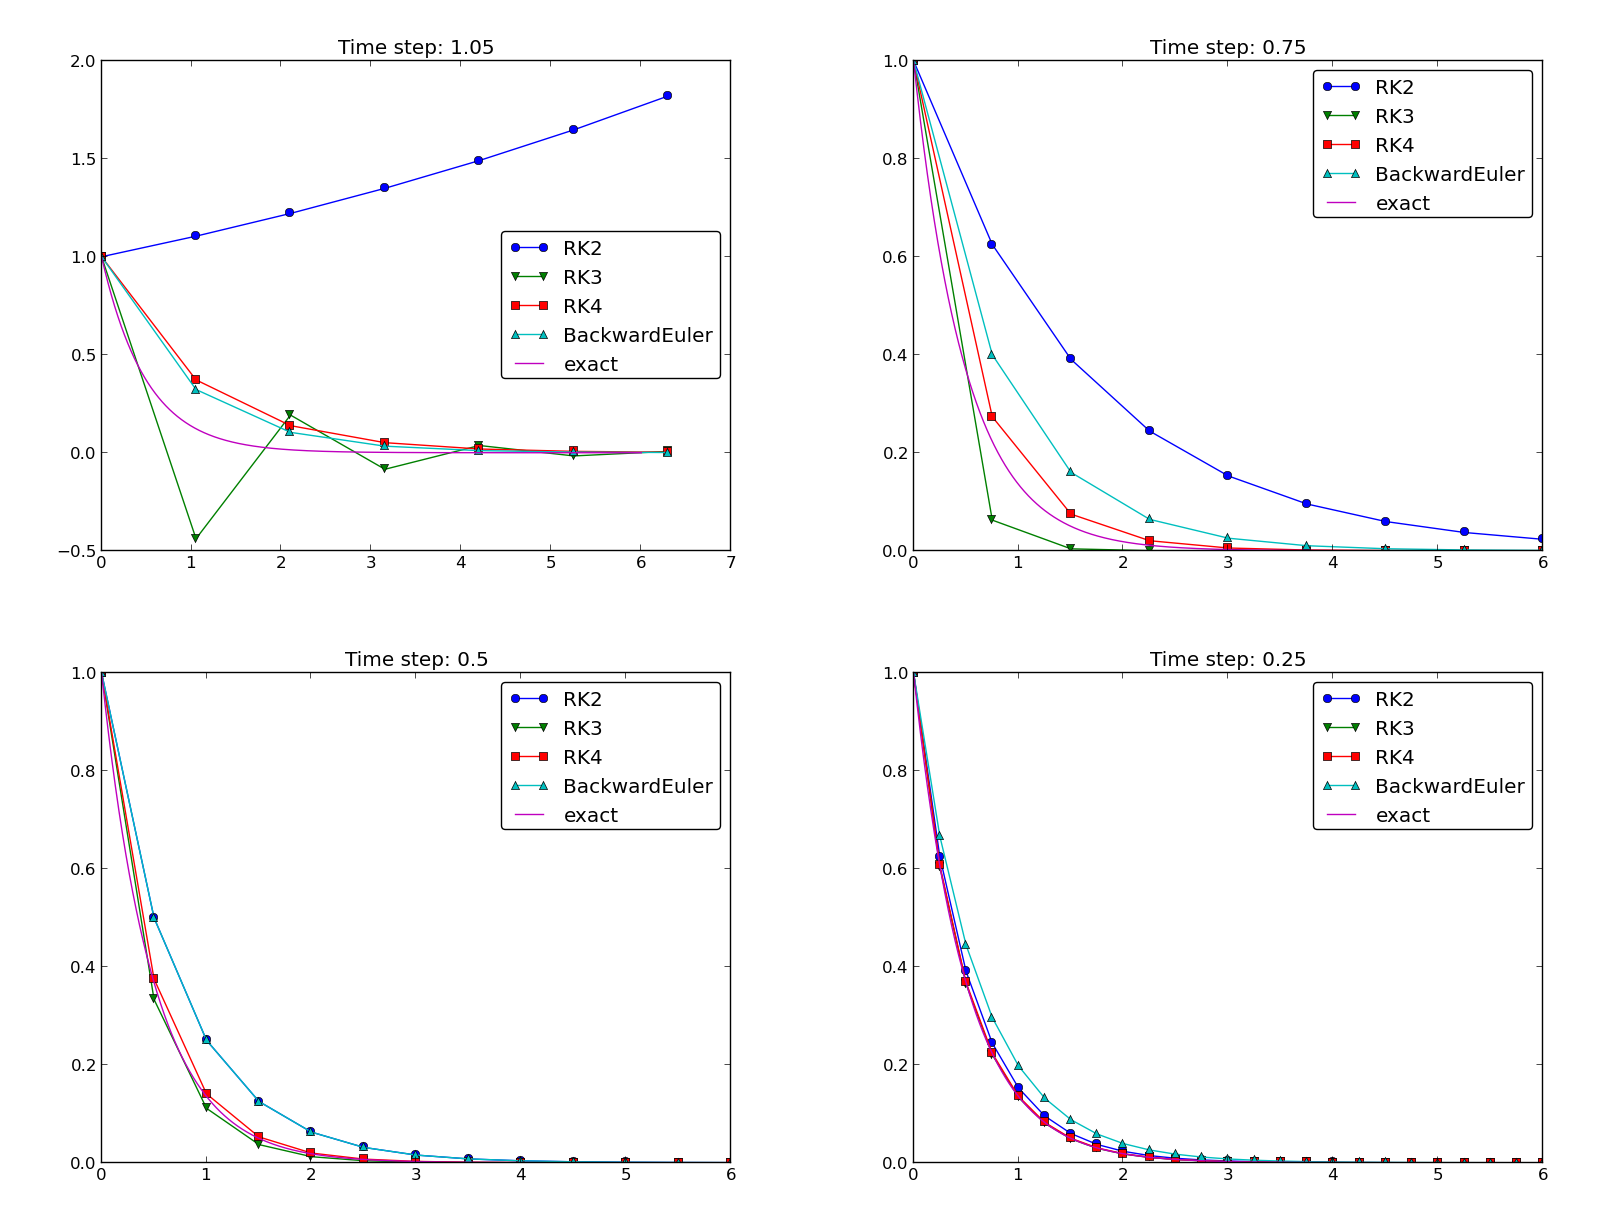
\includegraphics[width=1.1\linewidth]{fig-genz/decay_odespy1_png.png}}
  \caption{
  Behavior of different schemes for the decay equation. \label{decay:odespy:fig1}
  }
\end{figure}
%\clearpage % flush figures decay:odespy:fig1



The runs in Figure~\ref{decay:odespy:fig1}
and other experiments reveal that the 2nd-order Runge-Kutta
method (\texttt{RK2}) is unstable for $\Delta t>1$ and decays slower than the
Backward Euler scheme for large and moderate $\Delta t$ (see Exercise~\ref{decay:exer:RK2:Taylor:analysis} for an analysis).  However, for
fine $\Delta t = 0.25$ the 2nd-order Runge-Kutta method approaches
the exact solution faster than the Backward Euler scheme.  That is,
the latter scheme does a better job for larger $\Delta t$, while the
higher order scheme is superior for smaller $\Delta t$. This is a
typical trend also for most schemes for ordinary and partial
differential equations.

The 3rd-order Runge-Kutta method (\texttt{RK3}) also has artifacts in the form
of oscillatory behavior for the larger $\Delta t$ values, much
like that of the Crank-Nicolson scheme. For finer $\Delta t$,
the 3rd-order Runge-Kutta method converges quickly to the exact
solution.

The 4th-order Runge-Kutta method (\texttt{RK4}) is slightly inferior
to the Backward Euler scheme on the coarsest mesh, but is then
clearly superior to all the other schemes. It is definitely the
method of choice for all the tested schemes.


\paragraph{Remark about using the $\theta$-rule in Odespy.}
The Odespy package assumes that the ODE is written as $u^{\prime}=f(u,t)$ with
an $f$ that is possibly nonlinear in $u$. The $\theta$-rule for
$u^{\prime}=f(u,t)$ leads to
\[ u^{n+1} = u^{n} + \Delta t\left(\theta f(u^{n+1}, t_{n+1})
+ (1-\theta) f(u^{n}, t_{n})\right),\]
which is a \emph{nonlinear equation} in $u^{n+1}$. Odespy's implementation
of the $\theta$-rule (\texttt{ThetaRule}) and the specialized Backward Euler
(\texttt{BackwardEuler}) and Crank-Nicolson (\texttt{CrankNicolson}) schemes
must invoke iterative methods for
solving the nonlinear equation in $u^{n+1}$. This is done even when
$f$ is linear in $u$, as in the model problem $u^{\prime}=-au$, where we can
easily solve for $u^{n+1}$ by hand.  Therefore, we need to specify
use of Newton's method to solve the equations.
(Odespy allows other methods than Newton's to be used, for instance
Picard iteration, but that method is not suitable. The reason is that it
applies the Forward Euler scheme to generate a start value for
the iterations. Forward Euler may give very wrong solutions
for large $\Delta t$ values. Newton's method, on the other hand,
is insensitive to the start value in \emph{linear problems}.)


\subsection{Example: Adaptive Runge-Kutta methods}
\label{decay:fd2:adaptiveRK}

\index{adaptive time stepping}

Odespy also offers solution methods that can adapt the size of $\Delta t$
with time to match a desired accuracy in the solution. Intuitively,
small time steps will be chosen in areas where the solution is changing
rapidly, while larger time steps can be used where the solution
is slowly varying. Some kind of \emph{error estimator} is used to
adjust the next time step at each time level.

\index{ode45@{\rm\texttt{ode45}}} \index{Dormand-Prince Runge-Kutta 4-5 method}

A very popular adaptive method for solving ODEs is the Dormand-Prince
Runge-Kutta method of order 4 and 5. The 5th-order method is used as a
reference solution and the difference between the 4th- and 5th-order
methods is used as an indicator of the error in the numerical
solution.  The Dormand-Prince method is the default choice in MATLAB's
widely used \texttt{ode45} routine.

We can easily set up Odespy to use the Dormand-Prince method and
see how it selects the optimal time steps. To this end, we request
only one time step from $t=0$ to $t=T$ and ask the method to
compute the necessary non-uniform time mesh to meet a certain
error tolerance. The code goes like

\begin{pro}{cbg_blue1}{bar_blue1}\begin{Verbatim}[numbers=none,fontsize=\fontsize{9pt}{9pt},baselinestretch=0.95,xleftmargin=2mm]
import odespy
import numpy as np
import decay_mod
import sys
#import matplotlib.pyplot as plt
import scitools.std as plt

def f(u, t):
    return -a*u

def u_exact(t):
    return I*np.exp(-a*t)

I = 1; a = 2; T = 5
tol = float(sys.argv[1])
solver = odespy.DormandPrince(f, atol=tol, rtol=0.1*tol)

Nt = 1  # just one step - let the scheme find its intermediate points
t_mesh = np.linspace(0, T, Nt+1)
t_fine = np.linspace(0, T, 10001)

solver.set_initial_condition(I)
u, t = solver.solve(t_mesh)

# u and t will only consist of [I, u^Nt] and [0,T]
# solver.u_all and solver.t_all contains all computed points
plt.plot(solver.t_all, solver.u_all, 'ko')
plt.hold('on')
plt.plot(t_fine, u_exact(t_fine), 'b-')
plt.legend(['tol=%.0E' % tol, 'exact'])
plt.savefig('tmp_odespy_adaptive.png')
plt.show()
\end{Verbatim}
\end{pro}
\noindent

Running four cases with tolerances $10^{-1}$, $10^{-3}$, $10^{-5}$,
and $10^{-7}$, gives the results in Figure~\ref{decay:odespy:fig2}.
Intuitively, one would expect denser points in the beginning of
the decay and larger time steps when the solution flattens out.


\begin{figure}[!ht]  % decay:odespy:fig2
  \centerline{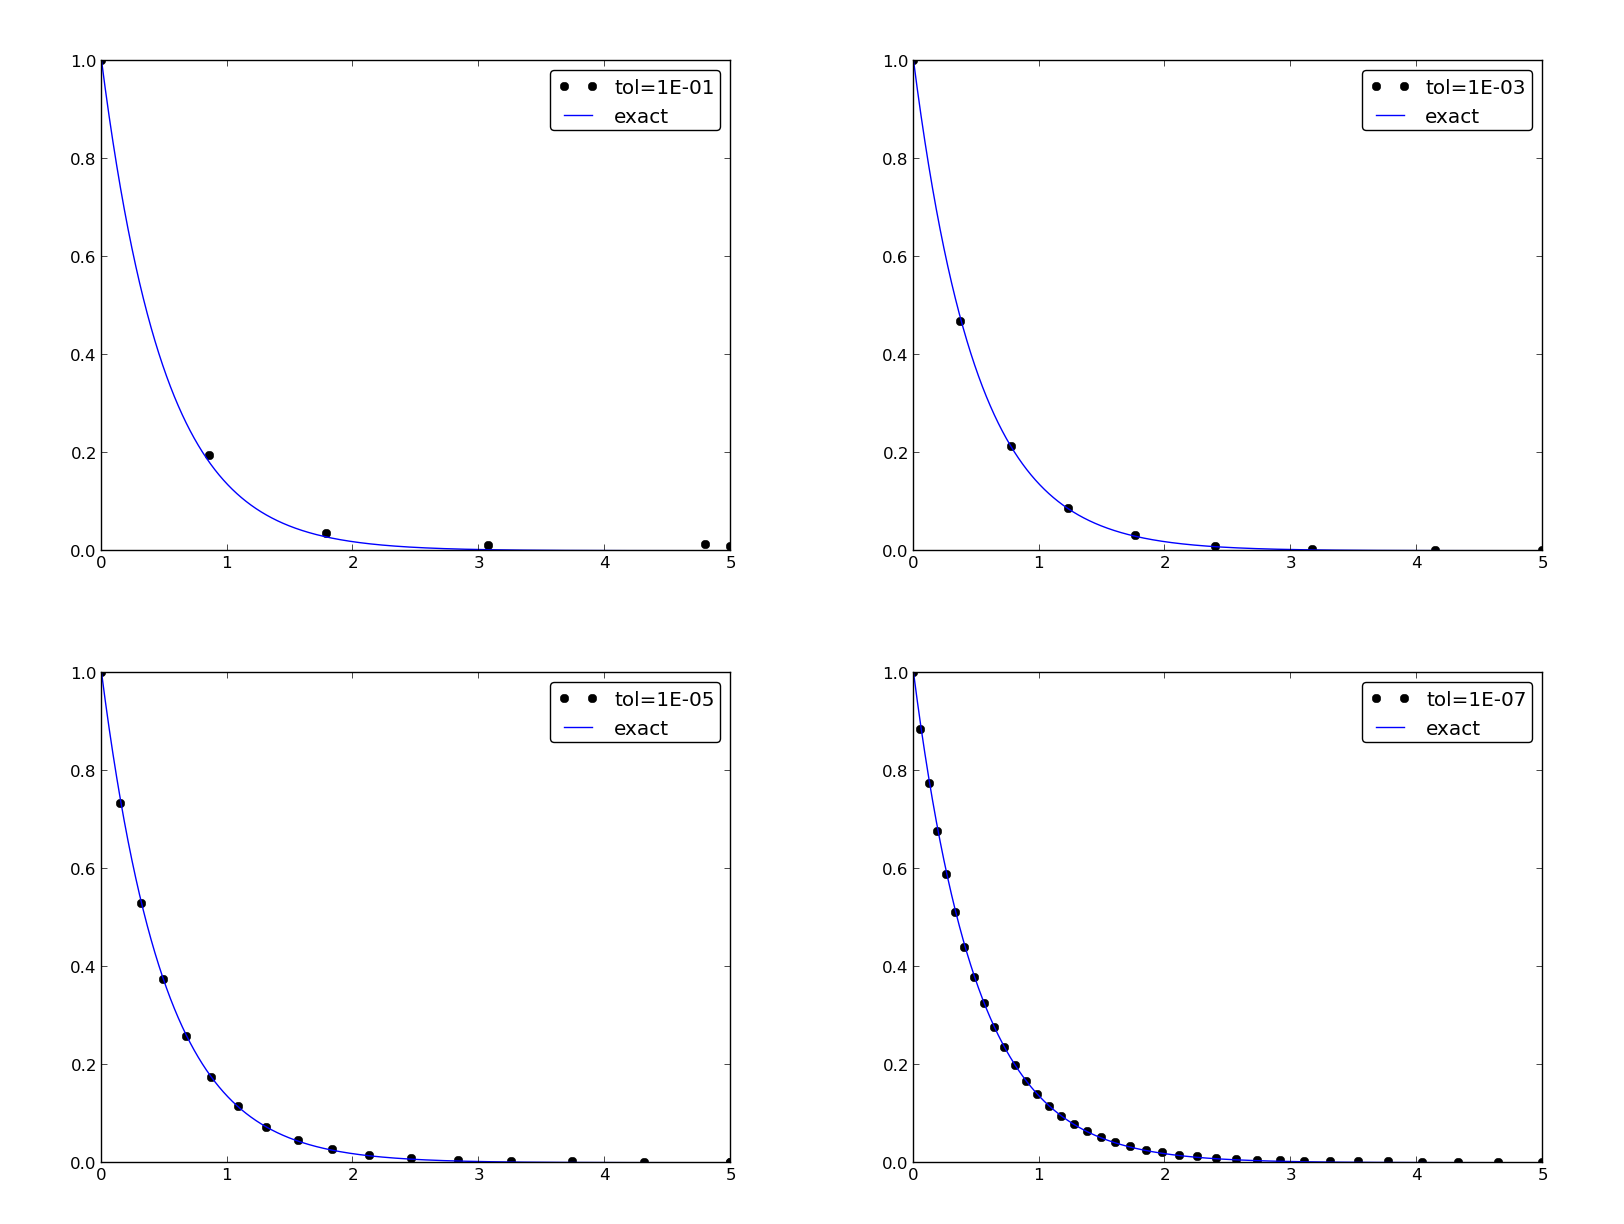
\includegraphics[width=1.2\linewidth]{fig-genz/decay_DormandPrince_adaptivity.png}}
  \caption{
  Choice of adaptive time mesh by the Dormand-Prince method for different tolerances. \label{decay:odespy:fig2}
  }
\end{figure}
%\clearpage % flush figures decay:odespy:fig2




\section{Exercises}



% --- begin exercise ---
\begin{doconceexercise}
\refstepcounter{doconceexercisecounter}

\subsection*{Exercise \thedoconceexercisecounter: Experiment with precision in tests and the size of $u$}

\label{decay:fd2:exer:precision}

It is claimed in Section~\ref{decay:MMS} that most numerical methods will
reproduce a linear exact solution to machine precision. Test this
assertion using the test function \Verb!test_linear_solution! in the
\href{{http://tinyurl.com/ofkw6kc/genz/decay_vc.py}}{\nolinkurl{decay_vc.py}} program.
Vary the parameter \texttt{c} from very small, via \texttt{c=1} to many larger values,
and print out the maximum difference between the numerical solution
and the exact solution. What is the relevant value of the tolerance
in the float comparison in each case?


% removed !bsol ... !esol environment (because of the command-line option --without_solutions)
\noindent Filename: \Verb!test_precision!.

\end{doconceexercise}
% --- end exercise ---




% --- begin exercise ---
\begin{doconceexercise}
\refstepcounter{doconceexercisecounter}

\subsection*{Exercise \thedoconceexercisecounter: Implement the 2-step backward scheme}

\label{decay:fd2:exer:bw2}

Implement the 2-step backward method (\ref{decay:fd2:bw:2step}) for the
model $u^{\prime}(t) = -a(t)u(t) + b(t)$, $u(0)=I$.  Allow the first step to
be computed by either the Backward Euler scheme or the Crank-Nicolson
scheme. Verify the implementation by choosing $a(t)$ and $b(t)$ such
that the exact solution is linear in $t$ (see Section~\ref{decay:MMS}). Show mathematically that a linear solution is indeed a
solution of the discrete equations.

Compute convergence rates (see Section~\ref{decay:convergence:rate}) in
a test case using $a=\hbox{const}$ and $b=0$, where we easily have an exact
solution, and determine if the choice of a first-order scheme
(Backward Euler) for the first step has any impact on the overall
accuracy of this scheme. The expected error goes like $\Oof{\Delta t^2}$.
\noindent Filename: \Verb!decay_backward2step!.

\end{doconceexercise}
% --- end exercise ---




% --- begin exercise ---
\begin{doconceexercise}
\refstepcounter{doconceexercisecounter}

\subsection*{Exercise \thedoconceexercisecounter: Implement the 2nd-order Adams-Bashforth scheme}

\label{decay:fd2:exer:AB2}

Implement the 2nd-order Adams-Bashforth method (\ref{decay:fd2:AB2})
for the decay problem $u^{\prime}=-a(t)u + b(t)$, $u(0)=I$, $t\in (0, T]$.
Use the Forward Euler method for the first step such that the overall
scheme is explicit. Verify the implementation using an exact
solution that is linear in time.
Analyze the scheme by searching for solutions $u^n=A^n$ when $a=\hbox{const}$
and $b=0$. Compare this second-order scheme to the Crank-Nicolson scheme.
\noindent Filename: \Verb!decay_AdamsBashforth2!.

\end{doconceexercise}
% --- end exercise ---




% --- begin exercise ---
\begin{doconceexercise}
\refstepcounter{doconceexercisecounter}

\subsection*{Exercise \thedoconceexercisecounter: Implement the 3rd-order Adams-Bashforth scheme}

\label{decay:fd2:exer:AB3}

Implement the 3rd-order Adams-Bashforth method (\ref{decay:fd2:AB3})
for the decay problem $u^{\prime}=-a(t)u + b(t)$, $u(0)=I$, $t\in (0, T]$.
Since the scheme is explicit, allow it to be started by two steps with
the Forward Euler method.  Investigate experimentally the case where
$b=0$ and $a$ is a constant: Can we have oscillatory solutions for
large $\Delta t$?
\noindent Filename: \Verb!decay_AdamsBashforth3!.

\end{doconceexercise}
% --- end exercise ---




% --- begin exercise ---
\begin{doconceexercise}
\refstepcounter{doconceexercisecounter}

\subsection*{Exercise \thedoconceexercisecounter: Analyze explicit 2nd-order methods}

\label{decay:exer:RK2:Taylor:analysis}

Show that the schemes (\ref{decay:fd2:RK2:s2}) and
(\ref{decay:fd2:Taylor2}) are identical in the case $f(u,t)=-a$, where
$a>0$ is a constant. Assume that the numerical solution reads
$u^n=A^n$ for some unknown amplification factor $A$ to be determined.
Find $A$ and derive stability criteria. Can the scheme produce
oscillatory solutions of $u^{\prime}=-au$? Plot the numerical and exact
amplification factor.
\noindent Filename: \Verb!decay_RK2_Taylor2!.

\end{doconceexercise}
% --- end exercise ---




% --- begin exercise ---
\begin{doconceexercise}
\refstepcounter{doconceexercisecounter}

\subsection*{Project \thedoconceexercisecounter: Implement and investigate the Leapfrog scheme}

\label{decay:fd2:exer:leapfrog1}

A Leapfrog scheme
for the ODE $u^{\prime}(t) = -a(t)u(t) + b(t)$ is defined by

\begin{equation}
\lbrack D_{2t}u = -au+b\rbrack^n\tp
\label{decay:fd2:exer:leapfrog1:scheme}
\end{equation}
A separate method is needed to compute $u^1$. The Forward Euler
scheme is a possible candidate.


\subex{a)}
Implement the Leapfrog scheme for the model equation.
Plot the solution in the case $a=1$, $b=0$, $I=1$,
$\Delta t = 0.01$, $t\in [0,4]$. Compare with the exact
solution $\uex(t)=e^{-t}$.

\subex{b)}
Show mathematically that a linear solution in $t$ fulfills the
Forward Euler scheme for the first step and the Leapfrog scheme
for the subsequent steps. Use this linear solution to verify
the implementation, and automate the verification through a test
function.

% --- begin hint in exercise ---

\paragraph{Hint.}
It can be wise to automate the calculations such that it is easy to
redo the calculations for other types of solutions. Here is
a possible \texttt{sympy} function that takes a symbolic expression \texttt{u}
(implemented as a Python function of \texttt{t}), fits the \texttt{b} term, and
checks if \texttt{u} fulfills the discrete equations:

\begin{cod}{cbg_blue1}\begin{Verbatim}[numbers=none,fontsize=\fontsize{9pt}{9pt},baselinestretch=0.95,xleftmargin=2mm]
import sympy as sym

def analyze(u):
    t, dt, a = sym.symbols('t dt a')

    print 'Analyzing u_e(t)=%s' % u(t)
    print 'u(0)=%s' % u(t).subs(t, 0)

    # Fit source term to the given u(t)
    b = sym.diff(u(t), t) + a*u(t)
    b = sym.simplify(b)
    print 'Source term b:', b

    # Residual in discrete equations; Forward Euler step
    R_step1 = (u(t+dt) - u(t))/dt + a*u(t) - b
    R_step1 = sym.simplify(R_step1)
    print 'Residual Forward Euler step:', R_step1

    # Residual in discrete equations; Leapfrog steps
    R = (u(t+dt) - u(t-dt))/(2*dt) + a*u(t) - b
    R = sym.simplify(R)
    print 'Residual Leapfrog steps:', R

def u_e(t):
    return c*t + I

analyze(u_e)
# or short form: analyze(lambda t: c*t + I)
\end{Verbatim}
\end{cod}
\noindent

% --- end hint in exercise ---

\subex{c)}
Show that a second-order polynomial in $t$ cannot be a solution of the discrete
equations. However, if a Crank-Nicolson scheme is used for the first
step, a second-order polynomial solves the equations exactly.


\subex{d)}
Create a manufactured solution $u(t)=\sin(t)$ for the ODE
$u^{\prime}=-au+b$.
Compute the convergence rate of the Leapfrog scheme using this
manufactured solution. The expected convergence rate of the
Leapfrog scheme is $\Oof{\Delta t^2}$. Does the use of a
1st-order method for the first step impact the convergence rate?

% A possible test case is
% $u^{\prime}=-au + b$, $u(0)=0$, where $\uex(t)=b/a + (I - b/a)e^{-at}$ if
% $a$ and $b$ are constants.

\subex{e)}
Set up a set of experiments to demonstrate that the Leapfrog scheme
(\ref{decay:fd2:exer:leapfrog1:scheme}) is associated with numerical artifacts
(instabilities). Document the main results from this investigation.

\subex{f)}
Analyze and explain the
instabilities of the Leapfrog scheme (\ref{decay:fd2:exer:leapfrog1:scheme}):

\begin{enumerate}
\item Choose $a=\mbox{const}$ and $b=0$. Assume that an exact solution
   of the discrete equations has
   the form $u^n=A^n$, where $A$ is an amplification factor to
   be determined. Derive an equation for $A$ by inserting $u^n=A^n$
   in the Leapfrog scheme.

\item Compute $A$ either by hand and/or with the aid of \texttt{sympy}.
   The polynomial for $A$ has two roots, $A_1$ and $A_2$. Let
   $u^n$ be a linear combination $u^n=C_1A_1^n + C_2A_2^n$.

\item Show that one of the roots is the reason for instability.

\item Compare $A$ with the exact expression, using a Taylor series approximation.

\item How can $C_1$ and $C_2$ be determined?
\end{enumerate}

\noindent
\subex{g)}
Since the original Leapfrog scheme is unconditionally unstable as time
grows, it demands some stabilization.  This can be done by filtering,
where we first find $u^{n+1}$ from the original Leapfrog scheme and
then replace $u^{n}$ by $u^n + \gamma (u^{n-1} - 2u^n +
u^{n+1})$, where $\gamma$ can be taken as 0.6.  Implement the filtered
Leapfrog scheme and check that it can handle tests where the original
Leapfrog scheme is unstable.


\noindent Filename: \Verb!decay_leapfrog!.

\end{doconceexercise}
% --- end exercise ---




% --- begin exercise ---
\begin{doconceexercise}
\refstepcounter{doconceexercisecounter}

\subsection*{Problem \thedoconceexercisecounter: Make a unified implementation of many schemes}

\label{decay:fd2:exer:uni}

Consider the linear ODE problem $u^{\prime}(t)=-a(t)u(t) + b(t)$, $u(0)=I$.
Explicit schemes for this problem can be written in the general form
\begin{equation}
u^{n+1} = \sum_{j=0}^m c_ju^{n-j},
\label{decay:analysis:exer:sumcj}
\end{equation}
for some choice of $c_0,\ldots,c_m$.
Find expressions for the $c_j$ coefficients in case of the
$\theta$-rule, the three-level backward scheme,
the Leapfrog scheme, the 2nd-order Runge-Kutta method,
and the 3rd-order Adams-Bashforth scheme.

Make a class \texttt{ExpDecay} that implements the
general updating formula (\ref{decay:analysis:exer:sumcj}).
The formula cannot be applied for $n < m$, and for those $n$ values, other
schemes must be used. Assume for simplicity that we just
repeat Crank-Nicolson steps until (\ref{decay:analysis:exer:sumcj}) can be used.
Use a subclass
to specify the list $c_0,\ldots,c_m$ for a particular method, and
implement subclasses for all the mentioned schemes.
Verify the implementation by testing with a linear solution, which should
be exactly reproduced by all methods.
\noindent Filename: \Verb!decay_schemes_unified!.

\end{doconceexercise}
% --- end exercise ---


% !split


\bibliographystyle{plain}
\bibliography{../papers}

% ------------------- end of main content ---------------

% #ifdef PREAMBLE
\cleardoublepage\phantomsection  % trick to get correct link to Index
\printindex

\end{document}
% #endif

